\documentclass[11pt]{amsart}

\usepackage[T1]{fontenc}
\usepackage{lmodern}
\usepackage{microtype}
\usepackage{booktabs}
\usepackage{array}
\usepackage{mathtools}
\usepackage{amssymb}
\usepackage{graphicx}
\usepackage{xcolor}
\usepackage{hyperref}

\hypersetup{
  colorlinks=true,
  linkcolor=blue!55!black,
  citecolor=blue!55!black,
  urlcolor=blue!55!black,
  pdftitle={Finite Positivity Certificates and a Cross-Endpoint Obstruction for a Riemann Xi-Defect Kernel},
  pdfauthor={Leonard van Hemert}
}

\newtheorem{theorem}{Theorem}[section]
\newtheorem{proposition}[theorem]{Proposition}
\newtheorem{lemma}[theorem]{Lemma}
\newtheorem{corollary}[theorem]{Corollary}
\theoremstyle{remark}
\newtheorem{remark}[theorem]{Remark}

\newcommand{\sinhc}{\operatorname{sinhc}}
\newcommand{\R}{\mathbb{R}}
\newcommand{\C}{\mathbb{C}}
\newcommand{\dd}{\,\mathrm{d}}

\title[Finite certificates and a cross-endpoint obstruction]{Finite Positivity Certificates and a Cross-Endpoint Obstruction for a Riemann $\Xi$-Defect Kernel}
\author{Leonard van Hemert}
\date{20 July 2026}

\begin{document}

\begin{abstract}
Let $\Xi(z)=\xi(\frac12+iz)$ and let $\Phi$ denote the positive even
Riemann theta kernel in its full-line Fourier representation.  We study the
two-variable cosine transform
\begin{align*}
C_y(x)&=\iint_{\R^2}(u+v)^2\sinhc(y(u+v))\Phi(u)\Phi(v)\\
&\hspace{5em}{}\times\cos(x(u-v))\dd u\dd v,
\qquad 0\leq y\leq\tfrac12.
\end{align*}
The Hermite--Biehler defect of $E=\Xi+i\Xi'$ equals $2yC_y(x)$.  Exact
endpoint formulas, strict raw-moment monotonicity, and a global Taylor
minorant for cosine lead to two results.  First, outward-rounded Arb
computation proves the zero-enumeration-free finite band
\[
C_y(x)>0\qquad
\left(0\leq y\leq\tfrac12,\ |x|\leq R_{10}\right),
\]
where
\[
7.0362433<R_{10}<7.0362434.
\]
Second, for every fixed $0\leq\varepsilon<1/2$, the initial positivity radii
of the associated cross-endpoint polynomial hierarchy have finite supremum.
The proof is analytic: the polynomial sections converge locally uniformly to
a mixed trigonometric--hyperbolic transform that tends to $-\infty$ on the
positive real axis.  Thus this fixed endpoint-mismatch mechanism cannot yield
unbounded positivity bands.  This obstruction does not disprove the Riemann
Hypothesis and does not apply to every moment or partition method.
\end{abstract}

\maketitle

\section{Introduction}

Write
\begin{equation}\label{eq:xi-definition}
\xi(s)=\frac12s(s-1)\pi^{-s/2}\Gamma(s/2)\zeta(s),
\qquad
\Xi(z)=\xi\!\left(\frac12+iz\right).
\end{equation}
The completed function satisfies
\begin{equation}\label{eq:functional-equation}
\xi(s)=\xi(1-s),
\end{equation}
and $\Xi$ is real entire and even.  The Jacobi transformation gives the
full-line representation
\begin{equation}\label{eq:fourier}
\Xi(z)=\int_{\R}\Phi(u)e^{izu}\dd u,
\end{equation}
where, in the normalization used here,
\begin{equation}\label{eq:phi}
\Phi(u)=\sum_{n=1}^{\infty}
\left(4\pi^2n^4e^{9|u|/2}-6\pi n^2e^{5|u|/2}\right)
e^{-\pi n^2e^{2|u|}}.
\end{equation}
For $u\geq0$, each summand is positive because
\[
4\pi^2n^4e^{9u/2}-6\pi n^2e^{5u/2}
=2\pi n^2e^{5u/2}\left(2\pi n^2e^{2u}-3\right)>0.
\]
The Jacobi transformation makes the extension in \eqref{eq:phi} even and
smooth.  The kernel also satisfies a bound
\begin{equation}\label{eq:decay}
0<\Phi(u)\leq C e^{9|u|/2}
\exp\!\left(-\frac{\pi}{2}e^{2|u|}\right)
\end{equation}
for a fixed $C>0$.

Moment inequalities, Fourier criteria, and Hermite--Biehler formulations for
$\Xi$ have a substantial history.  Csordas, Norfolk, and Varga proved
P\'olya--Tur\'an inequalities for Taylor coefficients \cite{CNV1986}.
Csordas and Varga proved strict concavity of
$t\mapsto\log\Phi(\sqrt t)$ and obtained broad moment inequalities
\cite{CV1988}.  Their later work developed Hermite--Biehler and generalized
Laguerre criteria \cite{CV1989,CV1990}.  Coffey and Csordas gave another proof
of logarithmic concavity and related moment inequalities \cite{CC2013}, while
Csordas studied positive-definite associated kernels and isolated global
positivity conditions equivalent to the Riemann Hypothesis \cite{C2015}.

The first contribution here combines moments at $y=0$ and $y=\frac12$ to
obtain one explicit polynomial lower bound for a two-variable defect kernel,
uniformly over the closed $y$-interval.  The endpoint moments are finite
combinations of derivatives of $\xi$ at $0$ and $\frac12$, so Arb can certify
them without locating zeros.  The first positive root gives the finite band.

The second contribution determines the fate of the same construction at all
orders.  For each fixed endpoint mismatch $0\leq\varepsilon<1/2$, the lower
polynomials converge to an explicit mixed transform.  The hyperbolic part
coming from $y=1/2$ has a strictly larger coefficient than the part coming
from $y=\varepsilon$, forcing the limit to $-\infty$.  Consequently the
certified radii of this hierarchy are bounded.  The conclusion is a no-go
theorem for this specific lower-polynomial mechanism, not for the Riemann
Hypothesis or for endpoint moments in general.

The zero consequence is not a record.  Platt and Trudgian rigorously verified
the Riemann Hypothesis through height $3\cdot10^{12}$ \cite{PT2021}.  The
interest of the present result lies in the moment certificate and its uniform
kernel inequality, rather than the small numerical height of the corollary.

\section{The defect kernel}

Set
\[
\sinhc t=
\begin{cases}
\sinh(t)/t,&t\neq0,\\
1,&t=0.
\end{cases}
\]
For $p=u+v$ and $q=u-v$, define
\begin{equation}\label{eq:W}
W_y(u,v)=p^2\sinhc(yp)\Phi(u)\Phi(v),
\qquad 0\leq y\leq\frac12,
\end{equation}
and
\begin{equation}\label{eq:C}
C_y(x)=\iint_{\R^2}W_y(u,v)\cos(xq)\dd u\dd v.
\end{equation}
For $y>0$, this equals the form
\[
C_y(x)=\iint_{\R^2}
\frac{p\sinh(yp)}{y}\Phi(u)\Phi(v)\cos(xq)\dd u\dd v.
\]

Estimate \eqref{eq:decay} shows that
\[
|p|^a|q|^b e^{|p|/2}\Phi(u)\Phi(v)
\]
is integrable for every fixed pair of nonnegative integers $a,b$.  Thus all
integrals and derivatives used below converge absolutely and locally
uniformly.  Fubini's theorem, differentiation under the integral, and the
limits at $y=0$ and $y=\frac12$ are valid.

\begin{lemma}[Defect identity]\label{lem:defect}
Let
\[
E(z)=\Xi(z)+i\Xi'(z),
\qquad
E^{\#}(z)=\overline{E(\bar z)}.
\]
Then
\begin{equation}\label{eq:defect}
|E(x+iy)|^2-|E^{\#}(x+iy)|^2=2yC_y(x)
\end{equation}
for real $x$ and $0\leq y\leq\frac12$.
\end{lemma}

\begin{proof}
Put $s=\frac12-y$ and
\[
P(s,x)=\xi(s+ix)\xi(s-ix)=|\Xi(x+iy)|^2.
\]
Multiply the Fourier integrals.  Symmetrization under $u\leftrightarrow v$
and under simultaneous sign reversal of $u$ and $v$ gives
\begin{equation}\label{eq:P-double}
P(s,x)=\iint_{\R^2}
\Phi(u)\Phi(v)\cosh(yp)\cos(xq)\dd u\dd v.
\end{equation}
Consequently,
\begin{equation}\label{eq:Py}
\frac{\partial P}{\partial y}(s,x)
=\iint p\sinh(yp)\Phi(u)\Phi(v)\cos(xq)\dd u\dd v
=yC_y(x).
\end{equation}

Because $\Xi$ is real entire,
$E^{\#}=\Xi-i\Xi'$.  Direct expansion yields
\[
|E|^2-|E^{\#}|^2
=-4\operatorname{Im}(\Xi'\overline{\Xi})
=2\frac{\partial}{\partial y}|\Xi(x+iy)|^2.
\]
Equation \eqref{eq:Py} proves \eqref{eq:defect}.
\end{proof}

At $y=0$, differentiation of \eqref{eq:Py} gives
\begin{equation}\label{eq:C0}
C_0(x)=2\left(\Xi'(x)^2-\Xi(x)\Xi''(x)\right).
\end{equation}

\section{Endpoint moments}

For $j\geq0$, define the raw moments
\begin{equation}\label{eq:A}
A_{2j}(y)=\iint_{\R^2}W_y(u,v)q^{2j}\dd u\dd v.
\end{equation}
Then
\begin{equation}\label{eq:C-derivatives}
C_y^{(2j)}(0)=(-1)^jA_{2j}(y),
\end{equation}
and $A_{2j}(y)>0$.

Define
\begin{equation}\label{eq:H}
H_{2j}(s)=\sum_{\ell=0}^{2j}(-1)^\ell
\binom{2j}{\ell}\xi^{(\ell)}(s)\xi^{(2j-\ell)}(s).
\end{equation}

\begin{lemma}[Moment identities]\label{lem:endpoints}
For $y>0$,
\begin{equation}\label{eq:A-H}
A_{2j}(y)=-\frac{H_{2j}'(\frac12-y)}{y}.
\end{equation}
The continuous endpoint values are
\begin{equation}\label{eq:endpoints}
A_{2j}(0)=H_{2j}''\!\left(\frac12\right),
\qquad
A_{2j}\!\left(\frac12\right)=-2H_{2j}'(0).
\end{equation}
\end{lemma}

\begin{proof}
Analytic continuation of \eqref{eq:fourier} gives
\[
\xi(s)=\int_{\R}\Phi(u)e^{(s-1/2)u}\dd u.
\]
Expanding $(u-v)^{2j}$ proves
\[
H_{2j}(s)=\iint_{\R^2}
e^{(s-1/2)p}q^{2j}\Phi(u)\Phi(v)\dd u\dd v.
\]
Equivalently, Leibniz differentiation gives
\[
\left.\partial_x^{2j}P(s,x)\right|_{x=0}=(-1)^jH_{2j}(s).
\]
Since $C_y=-P_s/y$, equations \eqref{eq:C-derivatives} and
\eqref{eq:A-H} follow.  The functional equation implies
\[
H_{2j}(1-s)=H_{2j}(s),
\qquad H_{2j}'(1/2)=0.
\]
Taylor expansion at $1/2$ gives the first endpoint formula; substituting
$y=1/2$ gives the second.
\end{proof}

\begin{lemma}[Strict raw-moment monotonicity]\label{lem:monotonicity}
For every $j\geq0$,
\[
0\leq y_1<y_2\leq\frac12
\quad\Longrightarrow\quad
A_{2j}(y_1)<A_{2j}(y_2).
\]
Consequently, with $m_{2j}(y)=A_{2j}(y)/A_0(y)$,
\begin{equation}\label{eq:cross-bounds}
\frac{A_{2j}(0)}{A_0(1/2)}
<m_{2j}(y)<
\frac{A_{2j}(1/2)}{A_0(0)}
\end{equation}
for every $y\in[0,1/2]$ and $j\geq1$.
\end{lemma}

\begin{proof}
For $p\neq0$,
\[
\sinhc(yp)=\sum_{r=0}^{\infty}
\frac{y^{2r}p^{2r}}{(2r+1)!}
\]
is strictly increasing for $y\geq0$.  The remaining factor in
\eqref{eq:A} is nonnegative and is positive away from measure-zero lines.
This proves strict monotonicity.  Applying the endpoint bounds separately to
the numerator and denominator gives \eqref{eq:cross-bounds}.  Equality would
require the numerator and denominator to attain opposite endpoints at the
same value of $y$, so both inequalities are strict even when $y$ is an
endpoint.
\end{proof}

\section{The degree-ten lower polynomial}

\begin{lemma}[Global cosine minorant]\label{lem:cosine}
For every real $r\neq0$,
\begin{equation}\label{eq:T10}
\cos r>
T_{10}(r):=
1-\frac{r^2}{2!}+\frac{r^4}{4!}-\frac{r^6}{6!}
+\frac{r^8}{8!}-\frac{r^{10}}{10!}.
\end{equation}
\end{lemma}

\begin{proof}
For $g=\cos-T_{10}$,
\[
g^{(10)}(r)=1-\cos r\geq0,
\]
and $g^{(k)}(0)=0$ for $0\leq k\leq9$.  Repeated integration proves
$g(r)\geq0$ for $r\geq0$.  The inequality is strict for $r>0$ because
$1-\cos r$ does not vanish identically on any interval $(0,r)$.  Evenness
handles negative $r$.
\end{proof}

For the five moments used below, set
\begin{equation}\label{eq:B}
\begin{aligned}
B_2&=\frac{A_2(1/2)}{A_0(0)},&
B_4&=\frac{A_4(0)}{A_0(1/2)},\\
B_6&=\frac{A_6(1/2)}{A_0(0)},&
B_8&=\frac{A_8(0)}{A_0(1/2)},\\
B_{10}&=\frac{A_{10}(1/2)}{A_0(0)}.
\end{aligned}
\end{equation}
Define
\begin{equation}\label{eq:Ptheta}
P_\theta(x)=
1-\frac{B_2x^2}{2!}+\frac{B_4x^4}{4!}
-\frac{B_6x^6}{6!}+\frac{B_8x^8}{8!}
-\frac{B_{10}x^{10}}{10!}.
\end{equation}

\begin{proposition}[Uniform polynomial lower bound]\label{prop:minorant}
For $0\leq y\leq\frac12$ and $x\neq0$,
\begin{equation}\label{eq:main-minorant}
\frac{C_y(x)}{A_0(y)}>P_\theta(x).
\end{equation}
\end{proposition}

\begin{proof}
Normalize $W_y\dd u\dd v$ by $A_0(y)$ and apply Lemma
\ref{lem:cosine}.  Strictness holds because $xq\neq0$ on a set of positive
measure.  We obtain
\[
\frac{C_y(x)}{A_0(y)}>
1-\frac{m_2(y)x^2}{2!}+\frac{m_4(y)x^4}{4!}
-\frac{m_6(y)x^6}{6!}+\frac{m_8(y)x^8}{8!}
-\frac{m_{10}(y)x^{10}}{10!}.
\]
For negative terms, use the upper bounds in \eqref{eq:cross-bounds}; for
positive terms, use the lower bounds.  This gives \eqref{eq:main-minorant}.
\end{proof}

\section{Certified endpoint arithmetic}

The certificate evaluates \eqref{eq:endpoints} from Taylor balls for
\begin{equation}\label{eq:xi-computational}
\xi(s)=(s-1)\pi^{-s/2}\Gamma(1+s/2)\zeta(s),
\end{equation}
which is algebraically identical to \eqref{eq:xi-definition} and analytic at
both centers $0$ and $1/2$.

Table \ref{tab:moments} lists ball centers.  At 269-bit Arb precision, the
largest radius among the twelve displayed values is $1.37\cdot10^{-67}$.

\begin{table}[ht]
\centering
\caption{Certified endpoint-moment ball centers.}
\label{tab:moments}
\scriptsize
\begin{tabular}{@{}c>{\raggedleft\arraybackslash}p{0.37\textwidth}>{\raggedleft\arraybackslash}p{0.37\textwidth}@{}}
\toprule
Moment & $A_{2j}(0)$ & $A_{2j}(1/2)$ \\
\midrule
$A_0$ & 0.02283966166888743667469247 & 0.02309570896612103381431025 \\
$A_2$ & 0.001890366586781360982949785 & 0.001909616896683607096775872 \\
$A_4$ & 0.000459720156209605774158694 & 0.000464013763611390134012507 \\
$A_6$ & 0.000182390894103604245533460 & 0.000183966337058884295480848 \\
$A_8$ & 0.000099156363571899705593806 & 0.000099954209940825929544209 \\
$A_{10}$ & 0.000067852553023503413540728 & 0.000068364291172414501807343 \\
\bottomrule
\end{tabular}
\end{table}

The resulting coefficient balls have centers
\begin{equation}\label{eq:B-values}
\begin{aligned}
B_2&=0.0836096840823574320891615416\ldots,\\
B_4&=0.0199050029979147510756695686\ldots,\\
B_6&=0.00805468748731450212309766654\ldots,\\
B_8&=0.00429328078723851344898443484\ldots,\\
B_{10}&=0.00299322696472082444610981628\ldots.
\end{aligned}
\end{equation}

Put $Q(t)=P_\theta(\sqrt t)$.  On $0\leq t\leq51$, the degree-four
Bernstein coefficient balls for $Q'$ have centers
\begin{equation}\label{eq:bernstein}
\begin{split}
&-0.0418048420411787160,\quad
-0.0206557763558942930,\\
&-0.0140554899445716895,\quad
-0.00787928068151705499,\\
&
-0.0159039318562651082.
\end{split}
\end{equation}
Every complete ball is negative.  Since Bernstein basis functions are
nonnegative on the unit interval, $Q'(t)<0$ for $0\leq t\leq51$.

For $t=51+r$, write
\[
Q'(51+r)=\sum_{j=0}^{4}c_jr^j.
\]
The coefficient-ball centers are
\begin{equation}\label{eq:tail-coefficients}
\begin{aligned}
c_0&=-0.0159039318562651082,\\
c_1&=-0.000629384405862592411,\\
c_2&=-0.0000327586169268804792,\\
c_3&=-0.000000415429458942178156,\\
c_4&=-0.000000004124265548832706.
\end{aligned}
\end{equation}
Again every complete ball is negative, so $Q'(t)<0$ for $t\geq51$.  Hence
\begin{equation}\label{eq:Q-monotone}
Q'(t)<0\qquad(t\geq0).
\end{equation}

The exact rational evaluation points satisfy the certified inequalities
\begin{align}
P_\theta(7.0362433)&>3.7223537277\cdot10^{-9}>0,
\label{eq:root-lower}\\
P_\theta(7.0362434)&<-1.7438217651\cdot10^{-8}<0.
\label{eq:root-upper}
\end{align}
Because $Q(0)=1$, \eqref{eq:Q-monotone} holds, and the leading coefficient
of $Q$ is negative, $P_\theta$ has exactly one positive zero.  Denote it by
$R_{10}$.  Then
\begin{equation}\label{eq:R10}
7.0362433<R_{10}<7.0362434,
\qquad
R_{10}=7.03624331759098920168\ldots.
\end{equation}

\begin{theorem}[Certified finite positivity band]\label{thm:finite-band}
For every $0\leq y\leq\frac12$,
\begin{equation}\label{eq:finite-band}
C_y(x)>0\qquad(|x|\leq R_{10}).
\end{equation}
\end{theorem}

\begin{proof}
For $0<|x|<R_{10}$, Proposition \ref{prop:minorant} and
$P_\theta(x)>0$ prove the claim.  At $|x|=R_{10}$, strictness in
\eqref{eq:main-minorant} gives
\[
\frac{C_y(R_{10})}{A_0(y)}>P_\theta(R_{10})=0.
\]
At $x=0$, $C_y(0)=A_0(y)>0$.  Evenness in $x$ completes the proof.
\end{proof}

\section{Finite zero consequence}

\begin{corollary}\label{cor:zeros}
If $\rho$ is a nontrivial zero of $\zeta$ with
$|\operatorname{Im}\rho|\leq R_{10}$, then
\[
\operatorname{Re}\rho=\frac12.
\]
\end{corollary}

\begin{proof}
At a zero of $\Xi$, the two functions $E$ and $E^{\#}$ have the same
modulus, so the left side of \eqref{eq:defect} vanishes.  If
$\rho=\beta+i\gamma$ with $\beta<1/2$, then
\[
z=\gamma+i(1/2-\beta)
\]
satisfies $\Xi(z)=\xi(\rho)=0$ and $0<\operatorname{Im}z<1/2$.  For
$|\gamma|\leq R_{10}$, Theorem \ref{thm:finite-band} and \eqref{eq:defect}
make the defect positive, a contradiction.  If $\beta>1/2$, the functional
equation and conjugation give the zero $1-\bar\rho$, with the same ordinate
and real part below $1/2$.
\end{proof}

At a real zero $x$ of $\Xi$, equation \eqref{eq:C0} becomes
$C_0(x)=2\Xi'(x)^2$.  Thus Theorem \ref{thm:finite-band} also implies simplicity
of any real $\Xi$-zero in the finite interval, without assuming simplicity.

\section{Failure for a generic positive kernel}

The proof uses positivity and decay in its analytic steps, but the numerical
moment profile is specific to the Riemann kernel.  Consider
\begin{equation}\label{eq:counterexample}
\Phi_\varepsilon(u)=
\psi_\varepsilon(u-1)+\psi_\varepsilon(u+1)
+\frac{13}{6}\psi_\varepsilon(u),
\qquad
\psi_\varepsilon(u)=e^{-2\cosh(u/\varepsilon)}.
\end{equation}
This kernel is smooth, positive, even, and double-exponentially decreasing.
Its Fourier transform factors as
\begin{equation}\label{eq:counterexample-FT}
\widehat{\Phi_\varepsilon}(z)=
2\varepsilon K_{i\varepsilon z}(2)
\left(2\cos z+\frac{13}{6}\right).
\end{equation}
With $\lambda=\log(3/2)$, one has $2\cosh\lambda=13/6$, so
\[
z=(2k+1)\pi\pm i\lambda
\]
are exact nonreal zeros and $0<\lambda<1/2$.

The failure appears already in the normalized moments.  Let
$a=13/6$ and let $m_{2j}^{(\varepsilon)}(y)$ denote the moments formed from
\eqref{eq:counterexample}.  Scaling each of the three bumps and applying
dominated convergence gives, for $j\geq1$,
\[
\frac{A_{2j}^{(\varepsilon)}(y)}{\varepsilon^2M^2}
\longrightarrow 4a\sinhc y,
\qquad
M=\int_{\R}e^{-2\cosh t}\dd t,
\]
while
\[
\frac{A_0^{(\varepsilon)}(y)}{\varepsilon^2M^2}
\longrightarrow 8\sinhc(2y)+4a\sinhc y.
\]
Therefore
\begin{equation}\label{eq:counterexample-moments}
\lim_{\varepsilon\to0}m_{2j}^{(\varepsilon)}(y)
=\frac{a}{2\cosh y+a}.
\end{equation}
At $y=\lambda$, this limit is $1/2$, which violates the Riemann-kernel
bound $m_2(y)<B_2=0.0836096840\ldots$ for all small enough $\varepsilon$.
At $y=0$, the limit is $13/25$.

For $0<\varepsilon\leq1/4$, the same family also satisfies
\[
\Phi_\varepsilon(1/2)^2<
\Phi_\varepsilon(0)\Phi_\varepsilon(1),
\]
so it is not log-concave.  Neither positivity nor rapid decay supplies the
endpoint ratios in \eqref{eq:B}.

\section{The cross-endpoint hierarchy}

The degree-ten theorem does not control the large-frequency sign of $C_y$.
The exact Taylor hierarchy makes the obstruction precise.  For $m\geq0$ set
\begin{equation}\label{eq:Sm}
S_m(y,x)=\sum_{j=0}^{2m+1}(-1)^j
\frac{m_{2j}(y)x^{2j}}{(2j)!}.
\end{equation}
The global Taylor inequality
$T_{4m+2}(r)<\cos r$ for $r\neq0$ gives
\begin{equation}\label{eq:Sm-lower}
S_m(y,x)<\frac{C_y(x)}{A_0(y)}
\qquad(x\neq0).
\end{equation}

\begin{proposition}[Exact hierarchy]\label{prop:exact-hierarchy}
Fix $\varepsilon>0$ and $R<\infty$.  Then $S_m$ converges uniformly to
$C_y(x)/A_0(y)$ on
\[
[\varepsilon,1/2]\times[-R,R].
\]
Moreover, $C_y(x)>0$ on this rectangle if and only if some $S_m$ is
uniformly positive there.
\end{proposition}

\begin{proof}
Estimate \eqref{eq:decay} gives a uniform exponential moment bound
\[
\sup_{\varepsilon\leq y\leq1/2}
\int e^{R|q|}\frac{W_y(u,v)}{A_0(y)}\dd u\dd v<\infty.
\]
Dominated convergence for the cosine series gives uniform convergence.  If
$C_y/A_0$ is positive on the compact rectangle, it has a positive minimum;
uniform convergence makes every sufficiently high section positive.  The
reverse implication follows from \eqref{eq:Sm-lower}, with the value at
$x=0$ equal to $1$.
\end{proof}

Thus divergence of the positivity radii for the exact sections is equivalent
to global open-strip positivity and supplies no weaker intermediate theorem.
The cross-endpoint hierarchy is more restrictive.  For $\varepsilon\geq0$,
define
\[
L_{2j}^{(\varepsilon)}=
\frac{A_{2j}(\varepsilon)}{A_0(1/2)},
\qquad
U_{2j}^{(\varepsilon)}=
\frac{A_{2j}(1/2)}{A_0(\varepsilon)},
\]
and
\begin{equation}\label{eq:Phat}
\widehat P_m^{(\varepsilon)}(x)=
1+
\sum_{\substack{1\leq j\leq2m+1\\ j\ \mathrm{even}}}
L_{2j}^{(\varepsilon)}\frac{x^{2j}}{(2j)!}
-
\sum_{\substack{1\leq j\leq2m+1\\ j\ \mathrm{odd}}}
U_{2j}^{(\varepsilon)}\frac{x^{2j}}{(2j)!}.
\end{equation}
Then
\[
\widehat P_m^{(\varepsilon)}(x)
<S_m(y,x)<\frac{C_y(x)}{A_0(y)}
\]
for $x\neq0$ and $\varepsilon\leq y\leq1/2$.  Theorem
\ref{thm:finite-band} is the case $m=2$, $\varepsilon=0$.

Let $\widehat R_m^{(\varepsilon)}$ be the initial positivity radius of
\eqref{eq:Phat}, namely the supremum of the initial interval on which it is
positive.  The next sections show that these radii cannot diverge for any
fixed $\varepsilon<1/2$.

\section{The exact mixed limit}

For fixed $y\in[0,1/2]$, define the hyperbolic transform
\begin{equation}\label{eq:G}
G_y(x)=C_y(ix)=\iint_{\R^2}W_y(u,v)\cosh(xq)\dd u\dd v.
\end{equation}
Although only real $x$ is needed below, $C_y(z)$ is entire in $z$.  Indeed,
for every $R>0$, estimate \eqref{eq:decay} gives
\[
\iint_{\R^2}W_y(u,v)e^{R|q|}\dd u\dd v<\infty
\]
uniformly for $0\leq y\leq1/2$.  Dominated convergence therefore gives the
absolutely and locally uniformly convergent series
\begin{align}
C_y(z)&=\sum_{j=0}^{\infty}(-1)^j
 A_{2j}(y)\frac{z^{2j}}{(2j)!},\label{eq:C-series}\\
G_y(z)&=\sum_{j=0}^{\infty}
 A_{2j}(y)\frac{z^{2j}}{(2j)!}.\label{eq:G-series}
\end{align}
Separating even and odd values of the index $j$ yields
\begin{align}
\sum_{j\ {\rm even}}A_{2j}(y)\frac{x^{2j}}{(2j)!}
 &=\frac{G_y(x)+C_y(x)}2,\label{eq:even-split}\\
\sum_{j\ {\rm odd}}A_{2j}(y)\frac{x^{2j}}{(2j)!}
 &=\frac{G_y(x)-C_y(x)}2.\label{eq:odd-split}
\end{align}

Fix $0\leq\varepsilon<1/2$ and abbreviate
\begin{equation}\label{eq:ab}
a=A_0(\varepsilon),\qquad b=A_0(1/2).
\end{equation}
Strict raw-moment monotonicity gives $0<a<b$.

\begin{proposition}[Mixed-limit formula]\label{prop:mixed-limit}
The polynomials $\widehat P_m^{(\varepsilon)}$ converge locally uniformly on
$\C$ to
\begin{equation}\label{eq:mixed-limit}
F_\varepsilon(x)=1-\frac ab
+\frac{G_\varepsilon(x)+C_\varepsilon(x)}{2b}
-\frac{G_{1/2}(x)-C_{1/2}(x)}{2a}.
\end{equation}
\end{proposition}

\begin{proof}
Apply \eqref{eq:even-split} to the positive even-index sum in
\eqref{eq:Phat} and \eqref{eq:odd-split} to its negative odd-index sum.
The $j=0$ term of the former is $a/b$, whereas the constant term of
$\widehat P_m^{(\varepsilon)}$ is defined to be one.  This produces the
essential correction $1-a/b$.  Local uniform convergence follows from
\eqref{eq:C-series}--\eqref{eq:G-series}.
\end{proof}

\section{Fixed endpoint mismatch forces bounded radii}

\begin{lemma}[Hyperbolic growth]\label{lem:hyperbolic-growth}
For each fixed $0\leq\varepsilon<1/2$, there are $c,\delta>0$ such that
\[
G_\varepsilon(x)\geq c\cosh(\delta x)\qquad(x\geq0).
\]
In particular, $G_\varepsilon(x)\to+\infty$ as $x\to+\infty$.
\end{lemma}

\begin{proof}
The density $W_\varepsilon$ is continuous and positive away from the null
line $u+v=0$.  Choose a compact rectangle on which $W_\varepsilon>0$ and
$|u-v|\geq\delta$ for some $\delta>0$.  Its $W_\varepsilon$-mass $c$ is
positive.  Restricting \eqref{eq:G} to this rectangle gives the bound.
\end{proof}

\begin{theorem}[Cross-endpoint obstruction]\label{thm:obstruction}
For every fixed $0\leq\varepsilon<1/2$,
\begin{equation}\label{eq:bounded-radii}
\sup_{m\geq0}\widehat R_m^{(\varepsilon)}<\infty.
\end{equation}
This statement is unconditional and does not assume the Riemann Hypothesis.
\end{theorem}

\begin{proof}
For each fixed real $p$, the function $y\mapsto\sinhc(yp)$ is increasing on
$[0,\infty)$.  Therefore
\[
W_{1/2}(u,v)\geq W_\varepsilon(u,v),
\qquad G_{1/2}(x)\geq G_\varepsilon(x)\quad(x\in\R).
\]
Positivity of the measures also gives $|C_y(x)|\leq A_0(y)$.  Formula
\eqref{eq:mixed-limit} consequently implies
\begin{equation}\label{eq:mixed-upper}
F_\varepsilon(x)
\leq 1-\frac ab+\frac{a}{2b}+\frac{b}{2a}
-\frac{b-a}{2ab}G_\varepsilon(x).
\end{equation}
The last coefficient is strictly negative because $a<b$, and Lemma
\ref{lem:hyperbolic-growth} shows that the final term tends to $-\infty$.
Hence $F_\varepsilon(x)\to-\infty$ as $x\to+\infty$.

Choose $X>0$ with $F_\varepsilon(X)<0$.  Proposition
\ref{prop:mixed-limit} gives
$\widehat P_m^{(\varepsilon)}(X)<0$ for every sufficiently large $m$, so
$\widehat R_m^{(\varepsilon)}\leq X$ for those $m$.  Each remaining
polynomial starts at one and has highest Taylor index $j=2m+1$, hence a
strictly negative leading coefficient.  It tends to $-\infty$ and has a
finite first positive zero.  Taking the maximum of $X$ and the finitely many
exceptional radii proves \eqref{eq:bounded-radii}.
\end{proof}

\begin{remark}[Endpoint distinction]\label{rem:endpoint}
The proof includes $\varepsilon=0$: $W_0=p^2\Phi(u)\Phi(v)$ is the continuous
endpoint weight and $A_0(0)>0$.  At $\varepsilon=1/2$, however, $a=b$ and
the coercive coefficient in \eqref{eq:mixed-upper} vanishes.  Then
\eqref{eq:mixed-limit} reduces to the exact normalized cosine transform.
The obstruction theorem neither proves nor disproves its global positivity.
\end{remark}

\section{Partitions and the RH-equivalence boundary}

On every fixed positive-width cell $[\alpha,\beta]\subset[0,1/2]$, using
positive coefficients from $\alpha$ and negative coefficients from $\beta$
repeats the proof of Theorem \ref{thm:obstruction}.  Thus a fixed finite
partition improves finite constants but does not remove endpoint mismatch.

Mesh refinement is different.  At fixed degree, continuity of the finitely
many moments makes the cellwise bounds converge to the exact Taylor section.
If degree and mesh are allowed to vary diagonally so that positivity is
certified on every compact rectangle
$[\varepsilon,1/2]\times[-R,R]$, Proposition
\ref{prop:exact-hierarchy} yields global open-strip defect positivity.
Through Lemma \ref{lem:defect} this is the Hermite--Biehler condition
equivalent to RH.  Such a diagonal assertion is therefore not an established
intermediate theorem; it reaches the original unresolved global condition.

Theorem \ref{thm:obstruction} blocks the fixed cross-endpoint hierarchy only.
It does not block exact moment sections.  Nor does it block adaptive schemes
with a new uniform estimate, or other approaches to RH.

\section{Higher-degree certified computation}

The analytic proof above is independent of numerical experimentation.  For
reproducibility and finite-scale diagnosis, an independent Arb implementation
nevertheless computed all 175 requested cases
\[
m=0,\ldots,20,25,30,40,50,
\qquad
\varepsilon\in\{0,1/4,1/8,1/16,1/32,10^{-2},10^{-3}\}.
\]
It certified 816 endpoint moments through $A_{202}$, an exact dyadic bracket
for every first positive root, and interval-Horner monotonicity up to that
root.  The successful full run used 700 decimal digits, a series cap of 205,
120 root-bisection bits, about $3.74$ seconds wall time, and approximately
$41.1$ MB maximum resident memory.  A 900-digit recomputation encloses every
degree-202 result.  The retained 180-digit run fails at $A_{120}(1/2)$ with
an indeterminate ball; it is recorded rather than suppressed.

At $m=50$, the extreme certified lower root endpoints are
\[
7.5367678370859\ldots\quad(\varepsilon=0),\qquad
7.7563175645352\ldots\quad(\varepsilon=1/4).
\]
These are finite certificates, not the proof of boundedness.

\begin{figure}[ht]
\centering
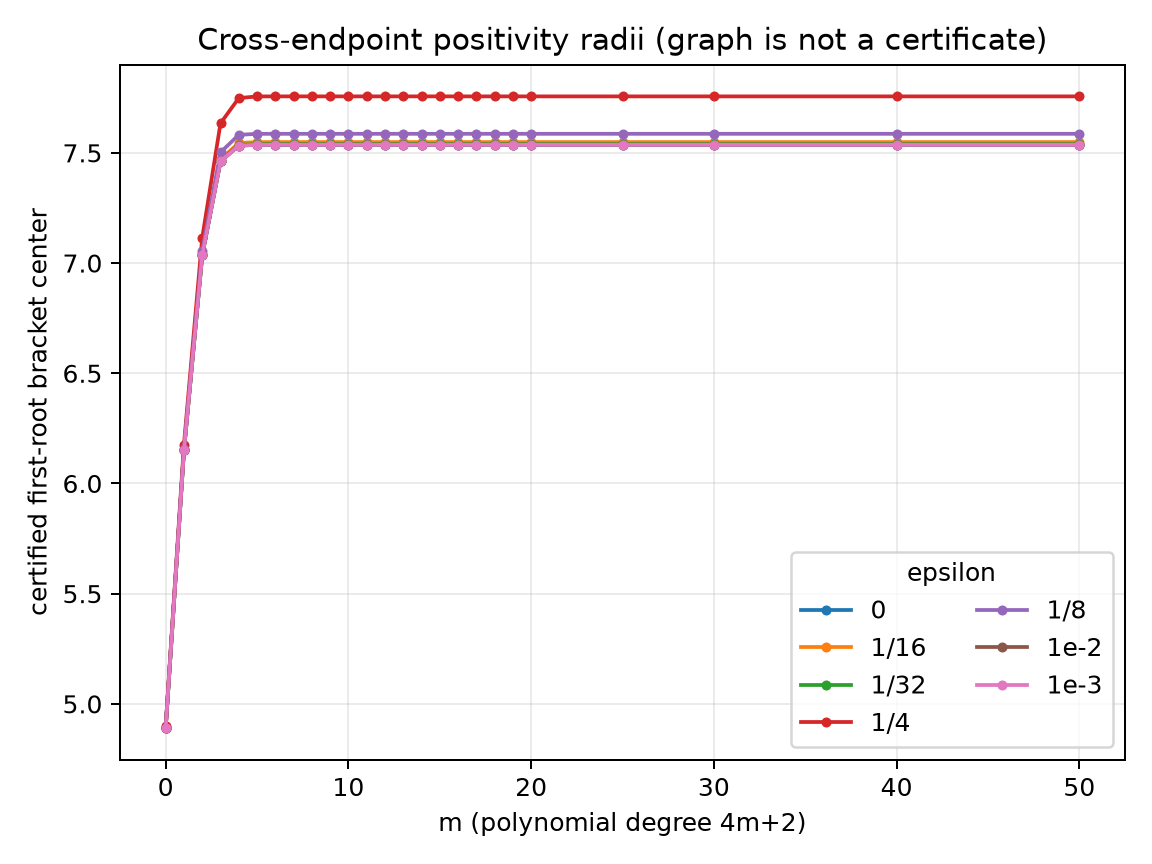
\includegraphics[width=0.92\textwidth]{../research/high_degree/radii.png}
\caption{Certified initial positivity radii for the computed degrees and
endpoint choices.  The plotted finite data diagnose the hierarchy but do not
establish an asymptotic law.  Theorem \ref{thm:obstruction} follows instead
from the exact mixed limit.}
\label{fig:radii}
\end{figure}

The clean-room program independently reconstructs the degree-10 endpoint
identities and root bracket.  A second implementation checks derivative
indexing, series caps, endpoint ratios, large-argument polynomial evaluation,
and precision loss as $\varepsilon\to0$.  These are internal reproducibility
and adversarial checks, not independent peer review.

\section{Reproducibility and certificate scope}

The public certificate evaluates Taylor balls for \eqref{eq:xi-computational}
at $0$ and $1/2$, forms \eqref{eq:H}, and extracts derivatives through order
$12$.  It uses \texttt{python-flint} 0.9.0, FLINT 3.6.0, 269-bit Arb precision, and a
formal-series cap of 18.  The cap exceeds the thirteen coefficients required
through degree 12.

The finite proof obligations are:
\begin{enumerate}
\item the twelve endpoint moment balls;
\item the five cross-endpoint ratios;
\item the five Bernstein signs in \eqref{eq:bernstein};
\item the five shifted-tail signs in \eqref{eq:tail-coefficients};
\item the two rational root-bracket signs.
\end{enumerate}
Arb implements midpoint-radius ball arithmetic with outward enclosures, so a
strict comparison succeeds only when the entire output ball lies on the
claimed side.  The computation uses no quadrature and no list of zeta zeros.
The analytic steps linking its finite values to $C_y$ are Lemmas
\ref{lem:defect}--\ref{lem:cosine} and Proposition \ref{prop:minorant}.

The repository records the exact dependency version, output, and SHA-256
checksums.  The command is
\begin{verbatim}
uv run --with python-flint==0.9.0 \
  python code/theta_moment_certificate.py
\end{verbatim}
Python optimization must remain disabled because program assertions encode
the sign obligations.  The higher-degree records and their independent
checks are reproduced by
\begin{verbatim}
uv run --with python-flint==0.9.0 \
  python research/high_degree/verify_results.py
PYTHONPATH=research/adversarial \
  uv run --with python-flint==0.9.0 \
  python -m unittest -v \
  research/adversarial/test_adversarial.py
\end{verbatim}

The dependency structure is:
\begin{enumerate}
\item the standard functional equation and Jacobi theta transformation give
      \eqref{eq:fourier}, positivity, and decay of $\Phi$;
\item those facts give absolute convergence, Lemmas
      \ref{lem:defect}--\ref{lem:cosine}, and the endpoint moments;
\item the finite Arb enclosures plus these analytic lemmas give Theorem
      \ref{thm:finite-band};
\item decay alone gives the entire series and Proposition
      \ref{prop:mixed-limit};
\item positivity, strict endpoint monotonicity, and the mixed limit give
      Theorem \ref{thm:obstruction};
\item no numerical radius, zero list, RH assumption, zero-simplicity
      assumption, or saddle-point heuristic enters the obstruction theorem.
\end{enumerate}

\section{Conclusion}

Endpoint derivatives of $\xi$ at $0$ and $1/2$, strict monotonicity of raw
moments, and a global cosine minorant produce an explicit lower polynomial for
$C_y/A_0$.  Arb certification of its coefficients and root proves the closed
finite band in Theorem \ref{thm:finite-band}.  At arbitrary degree, however,
fixed cross-endpoint normalization creates an imbalanced hyperbolic term.
The exact mixed limit tends to $-\infty$, and Theorem
\ref{thm:obstruction} proves that the resulting positivity radii remain
bounded for every fixed $\varepsilon<1/2$.

Thus the finite certificate is valid, while its fixed endpoint-mismatch
extension cannot prove RH.  This is not a theorem against RH, exact moment
sections, or every adaptive partition method.  The remaining global
open-strip positivity problem is unchanged and RH-equivalent.

\section*{Disclosure and licensing}

OpenAI Codex assisted with document preparation, computational orchestration,
and consistency checks.  The named author retains responsibility for the
mathematical claims and the released artifacts.  The paper and associated
scholarly materials are Copyright \textcopyright{} 2026 Leonard van Hemert.
All rights reserved; full terms appear in the repository \texttt{NOTICE}.
Repository software and certification scripts are AGPL-3.0-only.

\begin{thebibliography}{99}
\small

\bibitem{C2015}
G. Csordas,
\emph{Fourier transforms of positive definite kernels and the Riemann
$\xi$-function},
Comput. Methods Funct. Theory (2015),
\href{https://doi.org/10.1007/s40315-014-0105-8}{doi:10.1007/s40315-014-0105-8}.

\bibitem{CC2013}
M. W. Coffey and G. Csordas,
\emph{On the log-concavity of a Jacobi theta function},
Math. Comp. \textbf{82} (2013), 2265--2272,
\href{https://doi.org/10.1090/S0025-5718-2013-02681-6}{doi:10.1090/S0025-5718-2013-02681-6}.

\bibitem{CNV1986}
G. Csordas, T. S. Norfolk, and R. S. Varga,
\emph{The Riemann hypothesis and the Tur\'an inequalities},
Trans. Amer. Math. Soc. \textbf{296} (1986), 521--541,
\href{https://doi.org/10.1090/S0002-9947-1986-0846596-4}{doi:10.1090/S0002-9947-1986-0846596-4}.

\bibitem{CV1988}
G. Csordas and R. S. Varga,
\emph{Moment inequalities and the Riemann hypothesis},
Constr. Approx. \textbf{4} (1988), 175--198,
\href{https://doi.org/10.1007/BF02075457}{doi:10.1007/BF02075457}.

\bibitem{CV1989}
G. Csordas and R. S. Varga,
\emph{Fourier transforms and the Hermite--Biehler theorem},
Proc. Amer. Math. Soc. \textbf{107} (1989), 645--652,
\href{https://doi.org/10.1090/S0002-9939-1989-0982401-1}{doi:10.1090/S0002-9939-1989-0982401-1}.

\bibitem{CV1990}
G. Csordas and R. S. Varga,
\emph{Necessary and sufficient conditions and the Riemann hypothesis},
Adv. in Appl. Math. \textbf{11} (1990), 328--357,
\href{https://doi.org/10.1016/0196-8858(90)90013-O}{doi:10.1016/0196-8858(90)90013-O}.

\bibitem{PT2021}
D. J. Platt and T. S. Trudgian,
\emph{The Riemann hypothesis is true up to $3\cdot10^{12}$},
Bull. Lond. Math. Soc. \textbf{53} (2021), 792--797,
\href{https://doi.org/10.1112/blms.12460}{doi:10.1112/blms.12460}.

\end{thebibliography}

\end{document}
